\chapter{Realizace}
\label{realizace}
% promereni zapojeni jestli vse funguje 
% TODO + struktura firmware a provadeni digitalniho testu -> KAM TO ZARADIT? mozna do subsection realizace?
V této části bude popsána detailní realizace celého zařízení. V předchozích částech byly zmíněny základní požadavky na návrh celého vyčítacího rozhraní. Při výběru individuálních částí rozhraní byly tyto části respektovány. Dále jednotlivé části byly vybírány s ohledem na miniaturizaci rozhraní a spotřebu. Cílem návrhu bylo pokud co možno nejvíce funkčních bloků implementovat na základní desce. Prvním důvodem bylo, že druhá deska plošných spojů (chipboard) obsahuje detektor Timepix 2, který je v celém návrhu nejdůležitější a nejsložitější částí. Pokud by bylo vše implementováno na jedné desce plošných spojů, při jakémkoliv problému musí být vyměněna celá deska i s detektorem Timepix 2. Přitom při rozložení rozhraní na dvě desky plošných spojů dojde při případném problému k výměně jen základní desky. 
\par Druhým důvodem rozložení rozhraní na dvě desky plošných spojů je minimalizace rozměrů rozhraní. Za použití konektoru celé rozhraní zvýší své rozměry pouze na výšku o 3 mm přitom rozměry chipboardové desky mohou být stejné jako desky základní.

\section{Základní deska}
	\subsection{Napájení}
	Na základní desce je realizováno veškeré napájení potřebné pro celé výčítací rozhraní. Celkem jsou zde tři spínané synchronní buck regulátory. Konkrétně se jedná o regulátor MP2333H \cite{MPH2333} od společnosti Monolithic Power Systems. Regulátor pracuje v rozsahu vstupních napětí on 4.2 - 18 V. maximální výstupní proud jsou 3 A, spínací frekvence regulátoru je 1.2 MHz. Regulátor je možné pořídit v pouzdře SOT583, s rozměry 1.6x2 mm, které jsou pro úlohu minimalizace zařízení vyhovující. V tabulce \ref{tab:napajeni} můžete vidět seznam napětí dostupných na základní desce.
	\begin{table}[h!]
		\centering
		\begin{tabular}{ |P{3cm}||P{10cm}|  }
			\hline
			\multicolumn{2}{|c|}{Napájení základní desky vyčítacího rozhraní} \\
			\hline
			Napájení  & Popis\\ \hline \hline 
			+5V & Externí napájení vyčítacího rozhraní přes USB typu C. \\ \hline		
			+3V3 & Napájení pro mikrokontrolér, CPLD a další 3.3V periférie \\ \hline 		 
			+2V5 & Napájení vstupní a výstupní brány detektoru Timepix 2 \\ \hline
			+1V2 & Napájení jádra Timepix 2 a vstupní/výstupní brány CPLD.\\ \hline
		\end{tabular}
		\caption{Napájení základní desky vyčítacího rozhraní}
		\label{tab:napajeni}
	\end{table}
	Všechny napájení uvedené v tabulce \ref{tab:napajeni} jsou dostupné také na druhé desce, chipboardu. Více o propojení základní desky a chipboardové desky v části \ref{konektor}. Ukázkové zapojení jednoho ze tří spínaných regulátorů, můžete vidět na obrázku \ref{fig:mp2333h}. Konkrétně se jedná o zapojení, při kterém regulátor reguluje +5 V napájení na napájení +1.2 V.
	\begin{figure}[h!]
		\centering
		\captionsetup{justification=centering}
		\includegraphics[scale=0.80]{mp2333h.jpg}
		\caption{Zapojení regulátoru MP2333H} 
		\label{fig:mp2333h}
	\end{figure}
	\subsubsection{Napájecí sekvence}
	Napájecí sekvenci je možné vidět na zjednodušeném diagramu na obrázku \ref{fig:napajeci_sekvence}. Po připojení USB typu C do konektoru na základní dece je dostupné napájení +5 V. Těchto +5 V spíná první regulátor, který generuje na výstupu +3.3 V napájení. Pokud je toto výstupní napájení +3.3 V v pořádku, integrovaný obvod tuto informaci signalizuje pomocí pinu PG. Právě tento pin PG, signál PG\_3V3, je připojen na vstupní pin dalšího regulátoru v sérii a to na pin regulátoru generující výstupní napětí +2.5 V. Poslední regulátor s výstupním napětí +1.2 V je řízený z mikrokontroléru, jeho vstupní pin EN je propojen signálem EN\_1V2 s výstupní bránou mikrokontroléru.
	\begin{figure}[h!]
		\centering
		\captionsetup{justification=centering}
		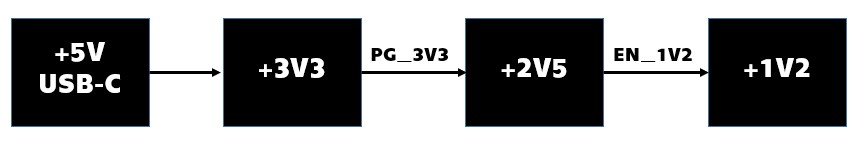
\includegraphics[scale=0.80]{napajeci_sekvence.jpg}
		\caption{Napájecí sekvence základní desky} 
		\label{fig:napajeci_sekvecne}
	\end{figure}
	\par Výstupní napětí spínaného regulátoru je nastaveno pomocí napěťového děliče ve zpětné vazbě regulátoru a dáno vztahem dle \ref{eq:Vout}. Kde $V_{REF}$ = 805 mV.
	\begin{equation}
		V_{OUT} = \frac{R1 \cdot V_{REF}}{R2} + V_{REF}
		\label{eq:Vout}
	\end{equation}

	\par Z obrázku \ref{fig:napajeci_sekvecne} je vidět, že spínaná stabilizátory pro +3.3 V a +2.5 V nejsou programově ovladatelné z mikrokontroléru. Spínaný stabilizátor +3.3 V, z mikrokontroléru řídit nelze, protože právě těchto +3.3 V je napájením pro vybraný mikrokontrolér. Možností jakým mimo jiné zajistit dodržení vhodného časování napájecí sekvence základní desky, je propojení PG signálu stabilizátoru +3.3 V na signál EN stabilizátoru +2.5 V. Další možností rozfázování napájecí sekvence je volba vhodného kondenzátoru mezi pinem SS a zemním pinem ze zapojení \ref{fig:mp2333h}. Kde $V_{REF}$ = 805 mV a $I_{SS}$ = 7.3 $\mu$A.
	\begin{equation}
		T_{SS}\,[ms] = \frac{2V_{REF} \cdot C_{SS} \,[nF]}{I_{SS}}
		\label{eq:Tss}
	\end{equation}
	Ze zapojení \ref{fig:mp2333h} a dosazení do vzorce \ref{eq:Tss} můžeme dopočítat, že rozběhový čas spínaného zdroje bude 1.4 ms. % TODO promerit Tss!!!
	
	\par Ochrana vstupního napájení bude popsána v části \ref{USB}. Pouze ve shrnutí, pokud dojde k jakýmkoliv podmínkám které by mohli elektricky ohrozit vyčítací rozhraní obvody z části \ref{USB} zajistí vypnutí napájení pomocí externího tranzistoru.
	
	%TODO spabilita napapájení

	\subsection{Mikrokontrolér}
	Mikrokontrolér pro tuto práci byl vybrán od firmy STMicroelectronics, přesněji mikrokontrolér s označením STM32U5A9NJH6Q \cite{STM32U5A9}. Právě tento mikrokontrolér byl vybrán s ohledem na požadavky očekávaná od vyčítacího rozhraní. V následující části budou uvedeny parametry vybraného mikrokontroléru
	%TODO napsat parametry MCU
	\par Prvním požadavkem na mikrokontrolér bylo, aby bylo možné komunikovat přes sériovou datovou linku s detektorem Timepix 2. V již popsané části textu \ref{Komunikacni rozhrani}, bylo zmíněno, že Timepix 2, dokáže komunikovat až na rychlostech 100 Mhz.  
	
	
	\subsection{Konverze logických úrovní}	
	\subsection{USB}
	\label{USB}

\section{Deska s Timepix 2}
	\subsection{Timepix 2}
	\subsubsection{Rozhraní pro připojení Timepix 2}
	\subsubsection{Napájení}
	\subsection{Vysokonapěťový zdroj}
		\subsubsection{Měření vysokého napětí}
	\subsection{Měření teploty}
	\subsection{Konektor}
	\label{konektor}
